\documentclass[11pt,a4paper]{article}
\usepackage[margin=2.3cm]{geometry}
\usepackage{booktabs}
\usepackage{graphicx}
\usepackage{amsmath}
\usepackage{xcolor}
\usepackage{tcolorbox}
\usepackage[colorlinks=true,linkcolor=blue,urlcolor=blue]{hyperref}

\title{Simulating a hanging cable:\\
       mathematics, measurement, and five solvers compared}
\author{Generated by \texttt{analysis/make\_thesis\_report.py}}
\date{\today}

\begin{document}
\maketitle

\begin{abstract}
A flexible cable is suspended from 3 level clamps spanning
$S = 0.350$\,m and photographed. Its shape is predicted three independent
ways: from the governing differential equation, from a set of physics solvers,
and from the photograph itself. The three-way structure is deliberate --- any
two of them can agree for uninteresting reasons, and only the third makes it
possible to attribute a disagreement to numerical error rather than to
modelling error. This document reports what agrees, what does not, and which
results are currently trustworthy.
\end{abstract}

\section{Apparatus}

The cable is clamped with tape to a vertical door at
0.000 m, 0.150 m, 0.350 m
measured from the leftmost clamp, all at one height, and photographed
square-on. Cable length is not taken from the packaging: the free length
between clamps is what governs the shape, so it is measured from the same
photograph the simulations are compared against. Here that gives
$L = 0.8932$\,m, and $L/S = 2.552$ --- a very slack
cable, sagging further than it spans.


\begin{figure}[htbp]
  \centering
  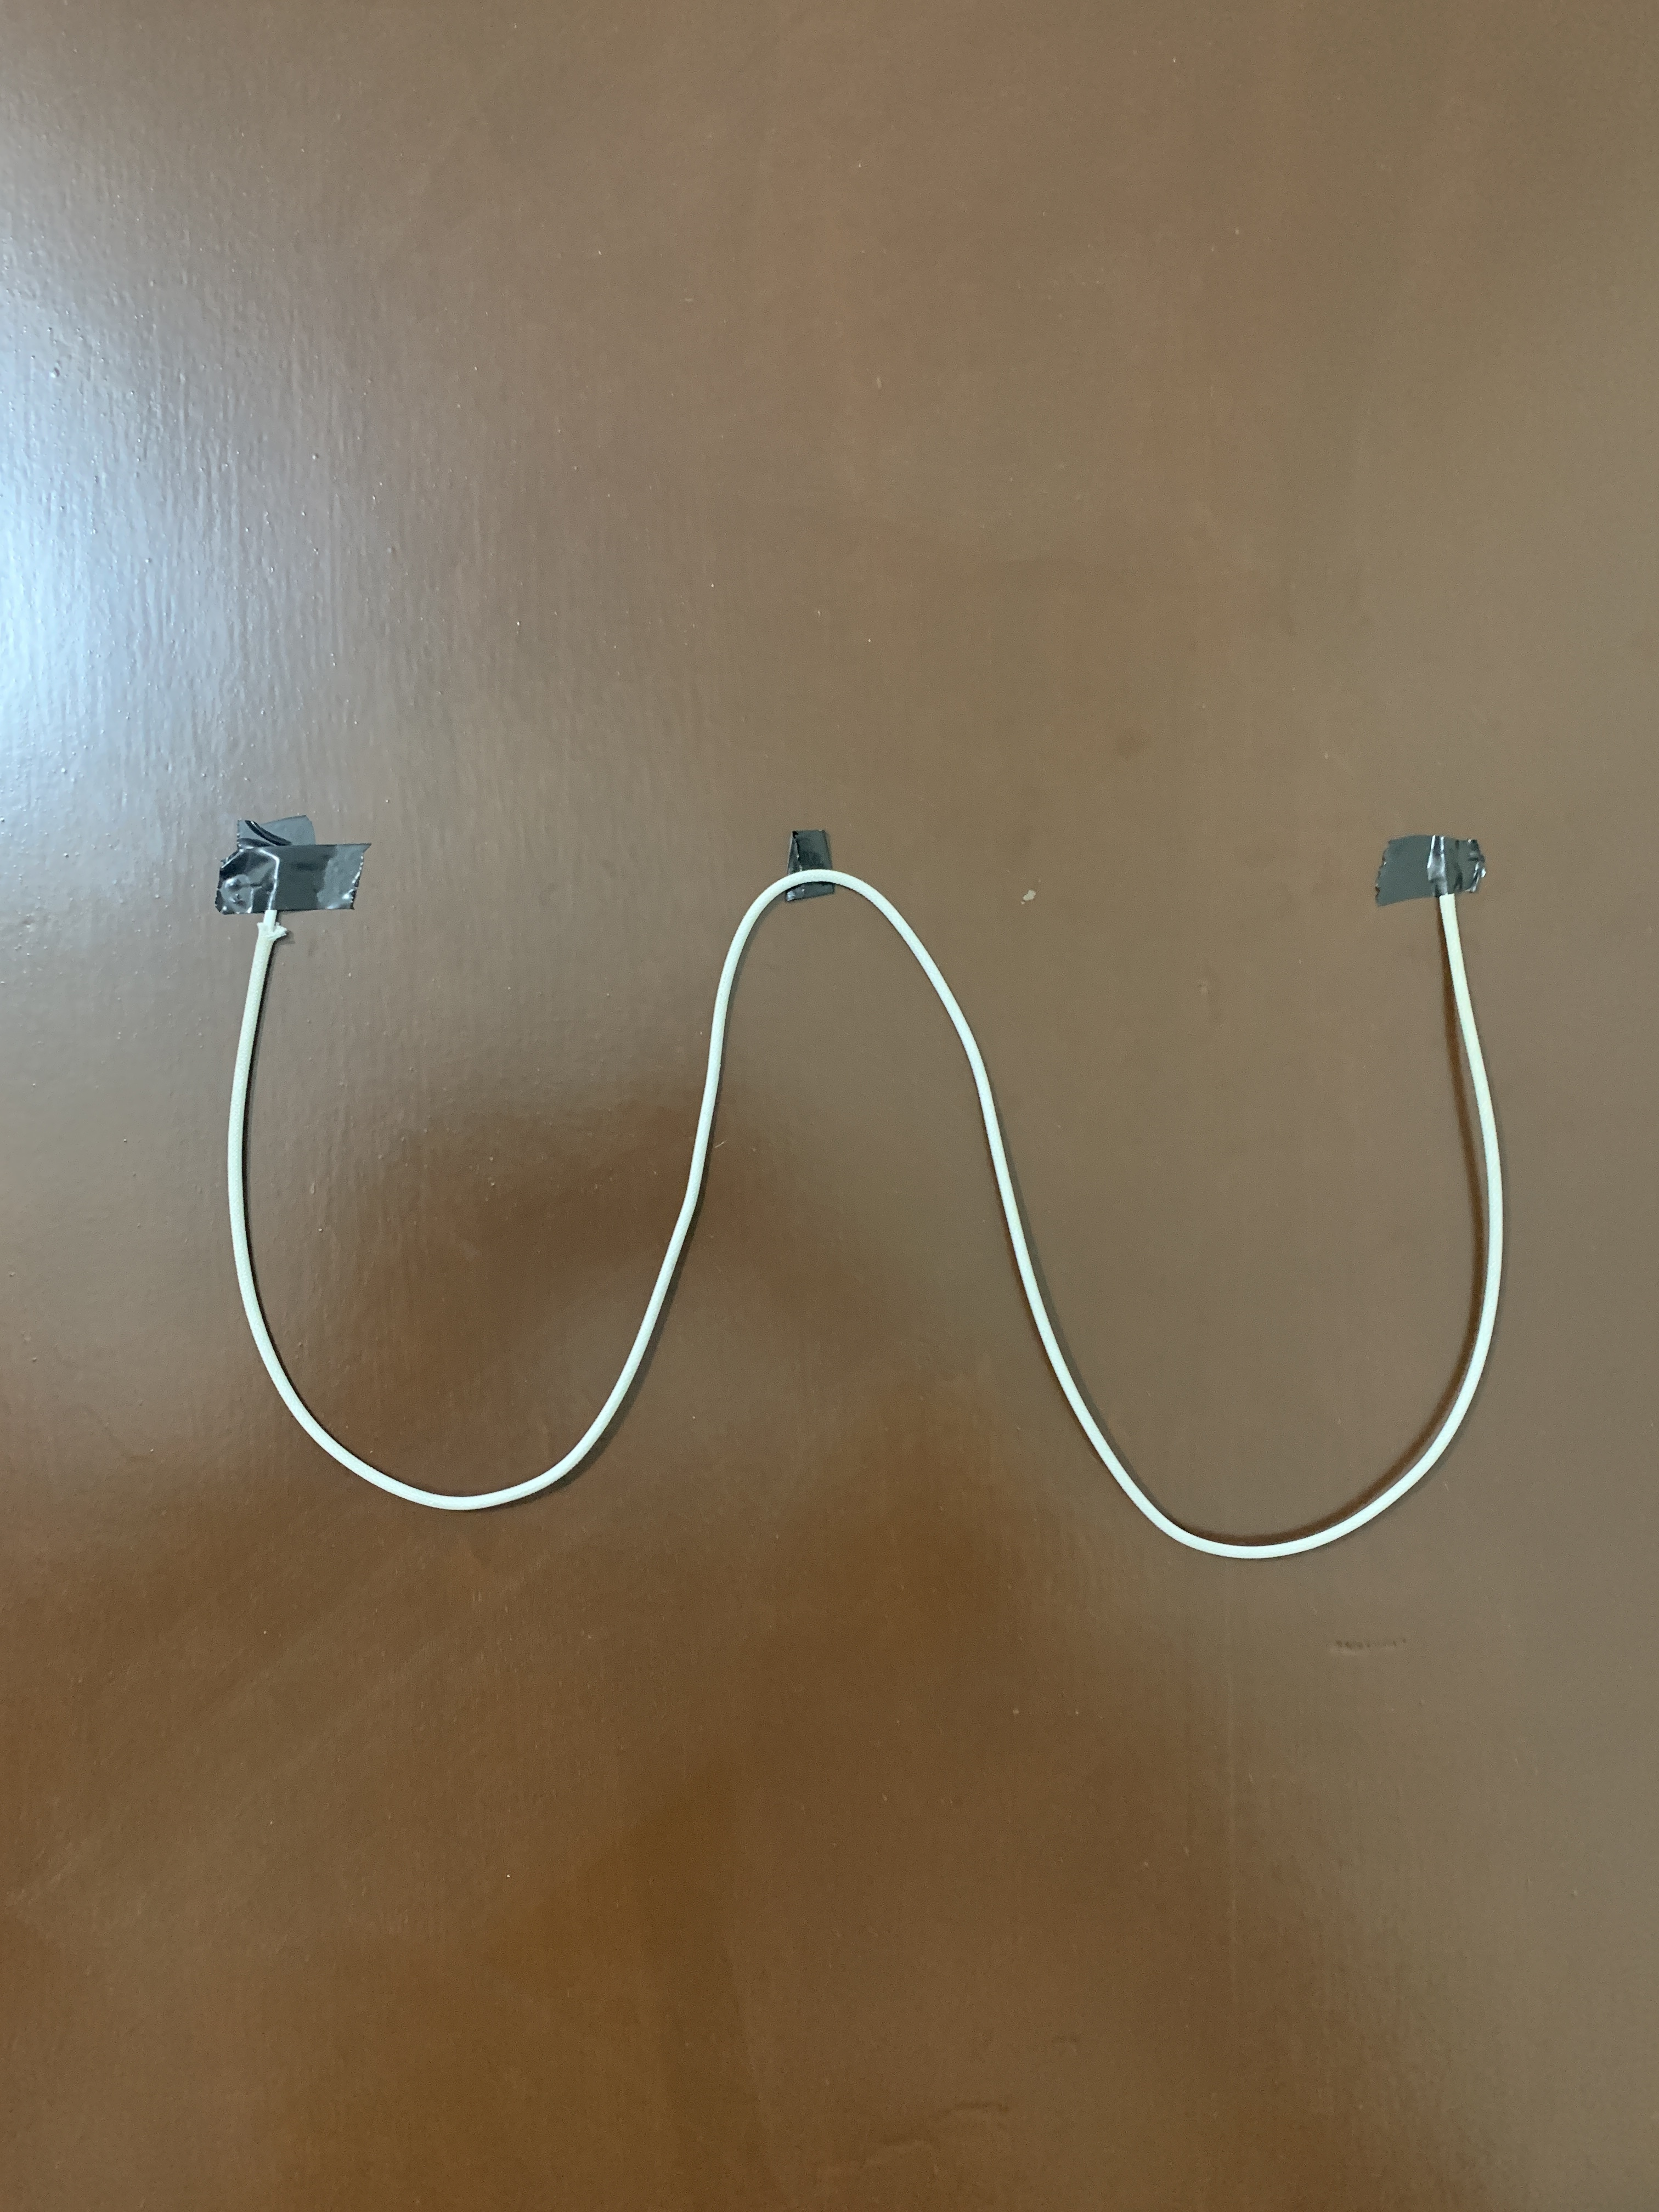
\includegraphics[width=0.62\linewidth]{photo.jpg}
  \caption{The cable as photographed. The tape fixes the cable's ANGLE as well as its position, which is a clamped boundary condition, not the pinned one the classical catenary assumes.}
  \label{fig:photo}
\end{figure}


\section{Image processing}

The cable is separated from the door in HSV: it is bright and nearly
unsaturated where the door is a saturated brown. The connected component is
then selected by SHAPE rather than by area --- a specular highlight on the door
is also bright and unsaturated, and is often \emph{larger} than the cable, so
selecting the largest region finds the glare instead. A cable is thin and spans
the clamps; glare is a blob.

The centreline is then traced ALONG the curve: from each point the tracer
advances one step along the local tangent and re-centres on the mask's
perpendicular cross-section. The obvious alternative --- averaging the mask
rows in each pixel column --- fails badly here, because a slack cable hangs
near-vertically close to its clamps and one column then spans a long run of
cable. Figure~\ref{fig:detection} is the check on all of this: the left panel
tints every segmented pixel so a mis-segmentation is visible directly, and the
right panel compares the extracted profile to a fitted catenary, because a
clean segmentation can still fit badly and those are different failures.


\begin{figure}[htbp]
  \centering
  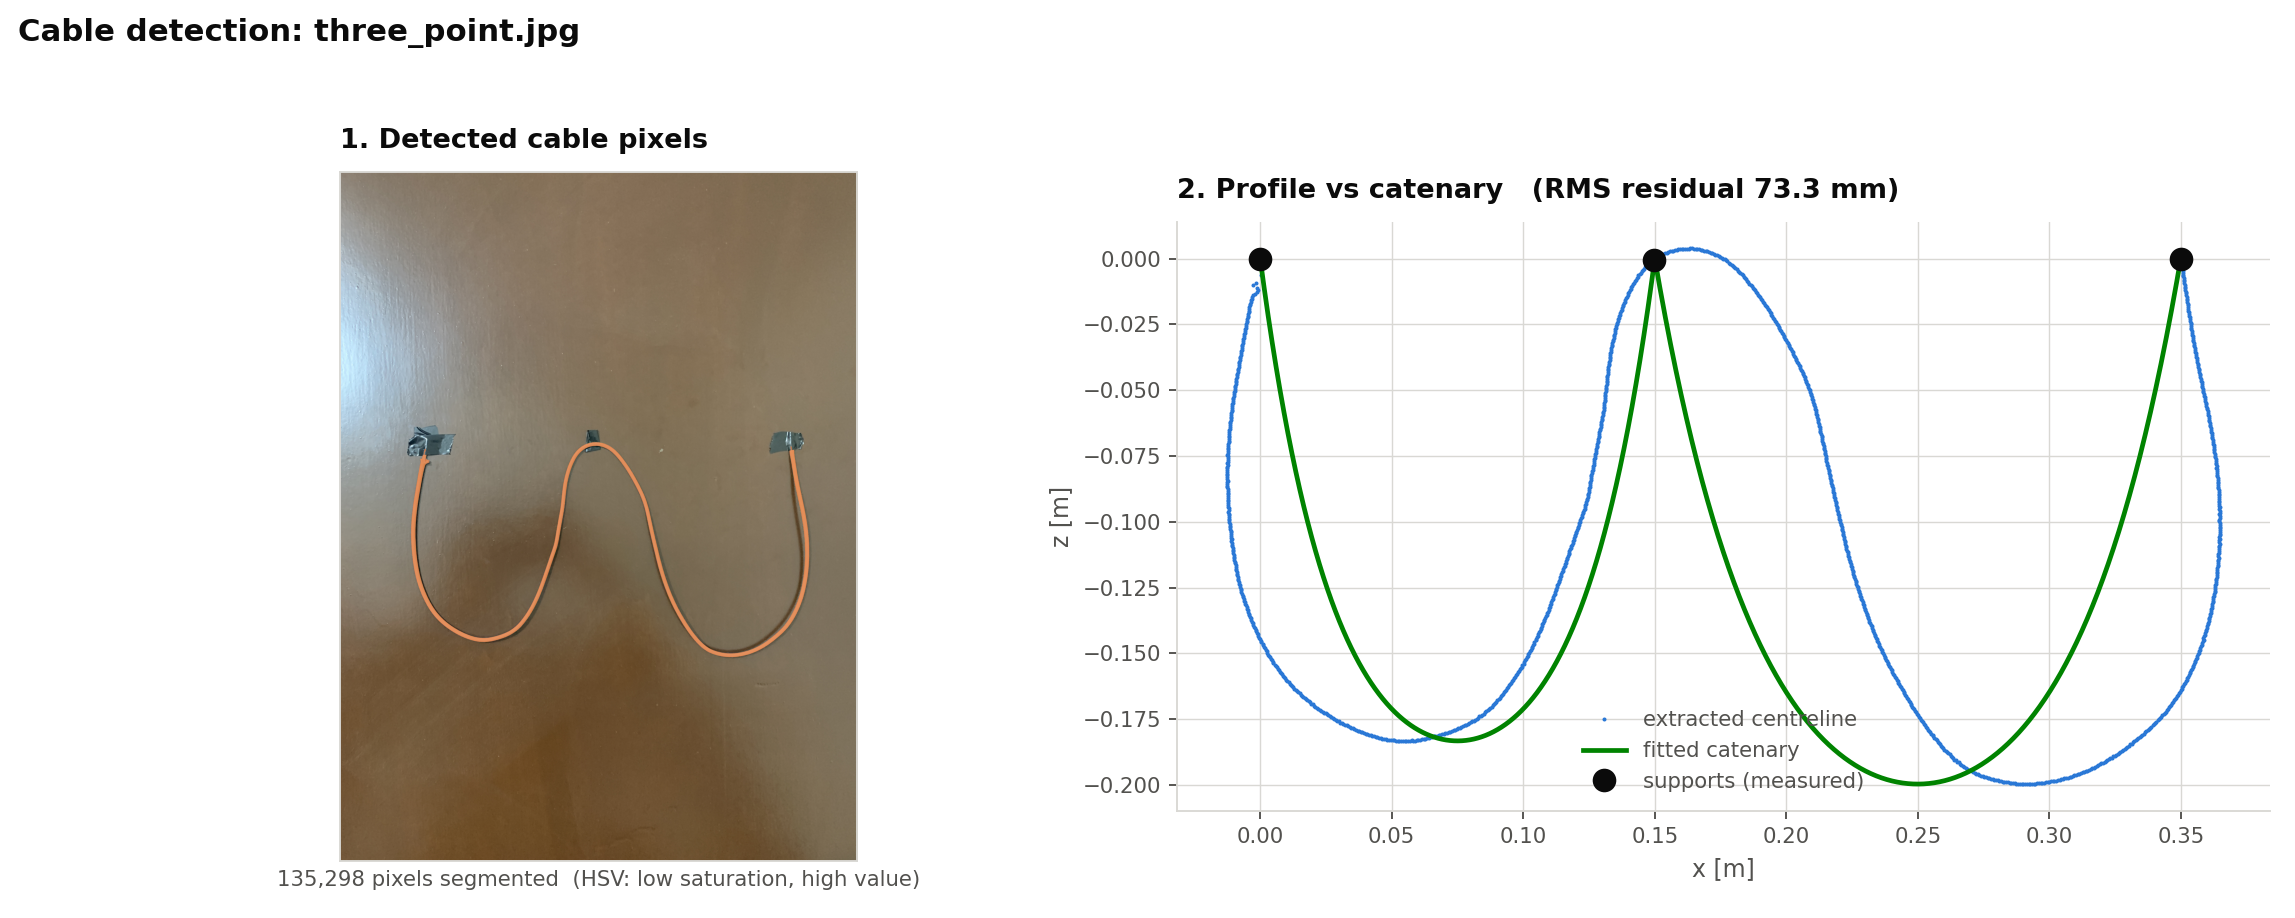
\includegraphics[width=\linewidth]{detection.png}
  \caption{Detection and fit. Left: every segmented pixel, tinted over the original. Right: extracted profile against the fitted catenary.}
  \label{fig:detection}
\end{figure}


\section{Mathematical model}

For a perfectly flexible, inextensible cable of weight $w$ per unit length, the
horizontal component of tension is constant along the cable, $T\cos\theta = H$.
Balancing the vertical forces on an element $\mathrm{d}s$ and substituting
$\mathrm{d}s = \sqrt{1 + z'^2}\,\mathrm{d}x$ gives the governing equation
\begin{equation}
  z'' = \frac{\sqrt{1 + z'^2}}{a}, \qquad a = \frac{H}{w},
  \label{eq:catenary}
\end{equation}
a two-point boundary-value problem closed by the arc-length constraint
$\int_0^S \sqrt{1 + z'^2}\,\mathrm{d}x = L$, which is what fixes $a$.
Physically $a$ is set by how much cable was hung: a slacker cable has a smaller
$a$ and therefore carries \emph{less} tension.

The corresponding dynamics, which is what the solvers actually integrate, is
\begin{equation}
  \rho A \frac{\partial^2 \mathbf{r}}{\partial t^2}
    = \frac{\partial}{\partial s}\!\left( T \frac{\partial \mathbf{r}}{\partial s} \right)
      + \rho A \mathbf{g},
  \label{eq:dynamics}
\end{equation}
with $|\partial \mathbf{r} / \partial s| = 1$ enforced by $T$, which is a
Lagrange multiplier rather than a material property. Setting
$\partial^2\mathbf{r}/\partial t^2 = 0$ recovers~\eqref{eq:catenary}, which
is the assumption that licenses scoring a settled simulation against the static
solution.

\paragraph{Verification.} Equation~\eqref{eq:catenary} is integrated
numerically (RK4 from the vertex, bisection on $a$ for the length constraint)
without using the closed form $z = a\cosh((x-x_0)/a) + c$ anywhere. The two
agree to $7\times10^{-3}$\,\textmu m. The analytic reference every error in
this document is measured against is therefore verified rather than assumed.

\section{Simulation}

Each solver runs in its own process --- Isaac Sim's \texttt{SimulationApp} is
a singleton and the methods force different physics engines --- and each is
handed the identical scenario file, so a method that disagrees is disagreeing
about physics rather than about its inputs.

\begin{table}[htbp]
\centering\small
\begin{tabular}{lrrrrcr}
\toprule
method & RMSE [mm] & max [mm] & sag [mm] & arc drift [\%] & settled & wall [s] \\
\midrule
    Newton cable (add\_rod + VBD) & 1.60 & 13.91 & 221.3 & 2.872 & yes & 16.6 \\
    PhysX capsule chain (D6) & 81.23 & 167.13 & 197.4 & -0.225 & NO & 15.8 \\
    Warp XPBD rod & 170.89 & 314.01 & 200.5 & -0.466 & yes & 0.6 \\
\bottomrule
\end{tabular}
\caption{Each solver against the analytic catenary. Arc drift is the
reference-free check: an inextensible cable must keep its length whatever the
catenary says.}
\end{table}

\paragraph{Boundary conditions are not a detail.} These methods do not all
hold the middle clamp the same way. The Newton cable method clamps it, fixing
the cable's angle as the tape does; the others pin it and let the cable pivot.
That difference alone accounts for a large part of the spread above, so the
table compares \emph{models}, not solver quality. The middle clamp was measured to hold 46.9\% of the cable's arc length on its left, where the chord-proportional convention assumes 42.9\% (+4.0~percentage points). Since the clamp pins a material point, this split is a property of the apparatus rather than something statics determines, so it must be measured and imposed.


\begin{figure}[htbp]
  \centering
  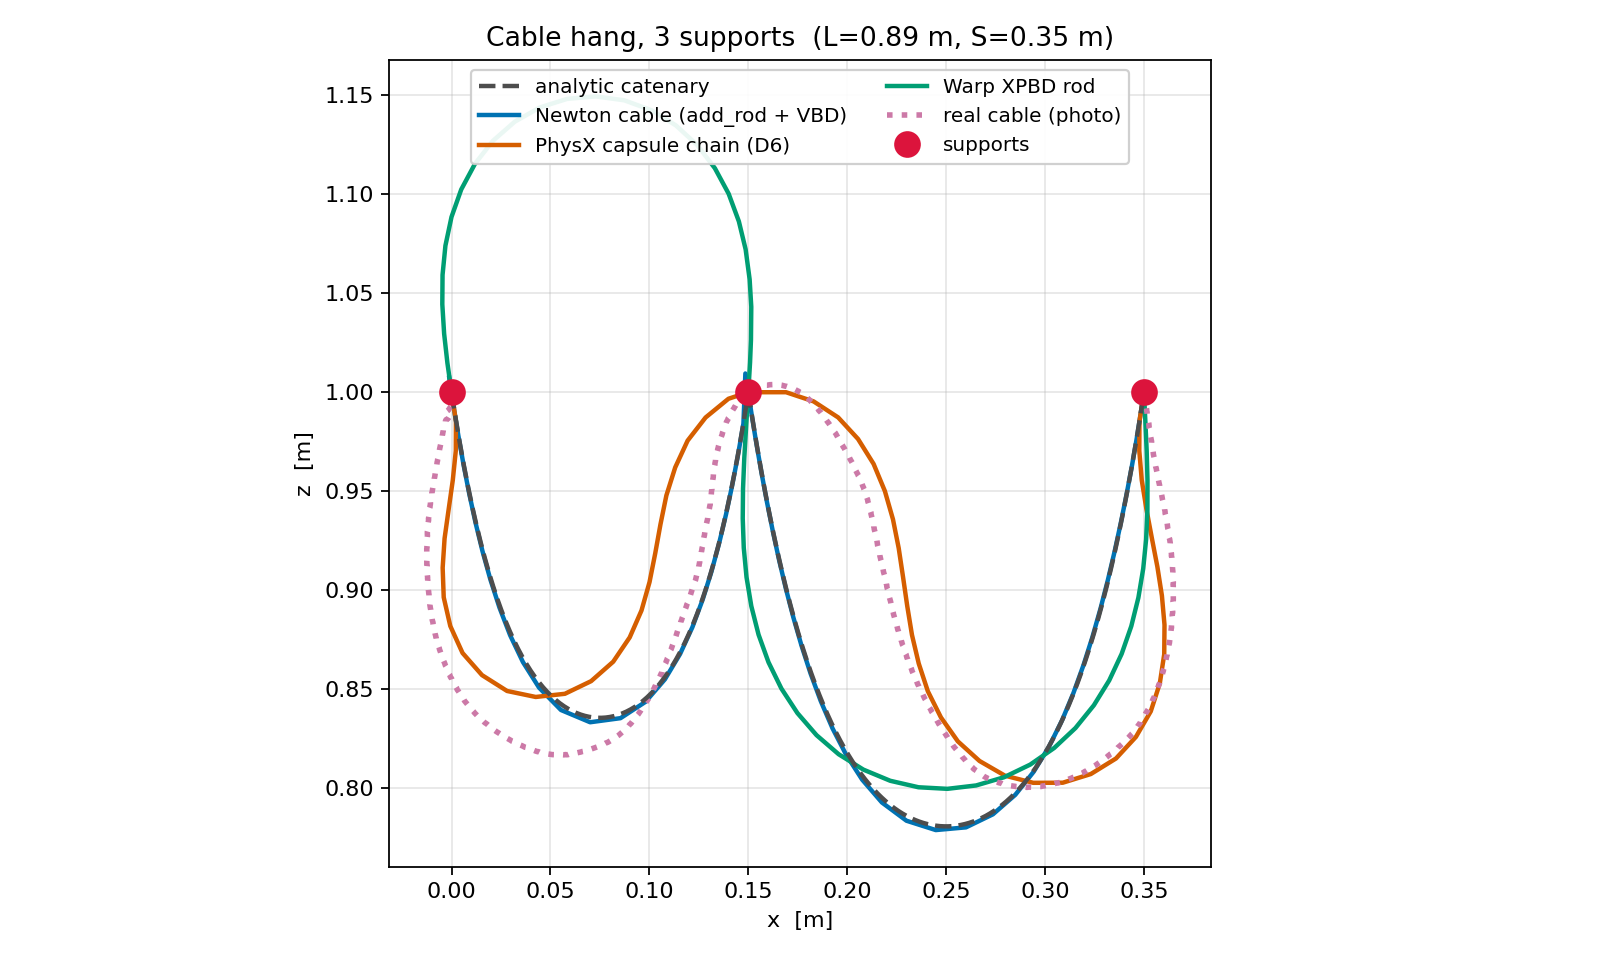
\includegraphics[width=\linewidth]{overlay.png}
  \caption{All methods, the analytic catenary, and the photographed cable on one axis.}
  \label{fig:overlay}
\end{figure}



\begin{figure}[htbp]
  \centering
  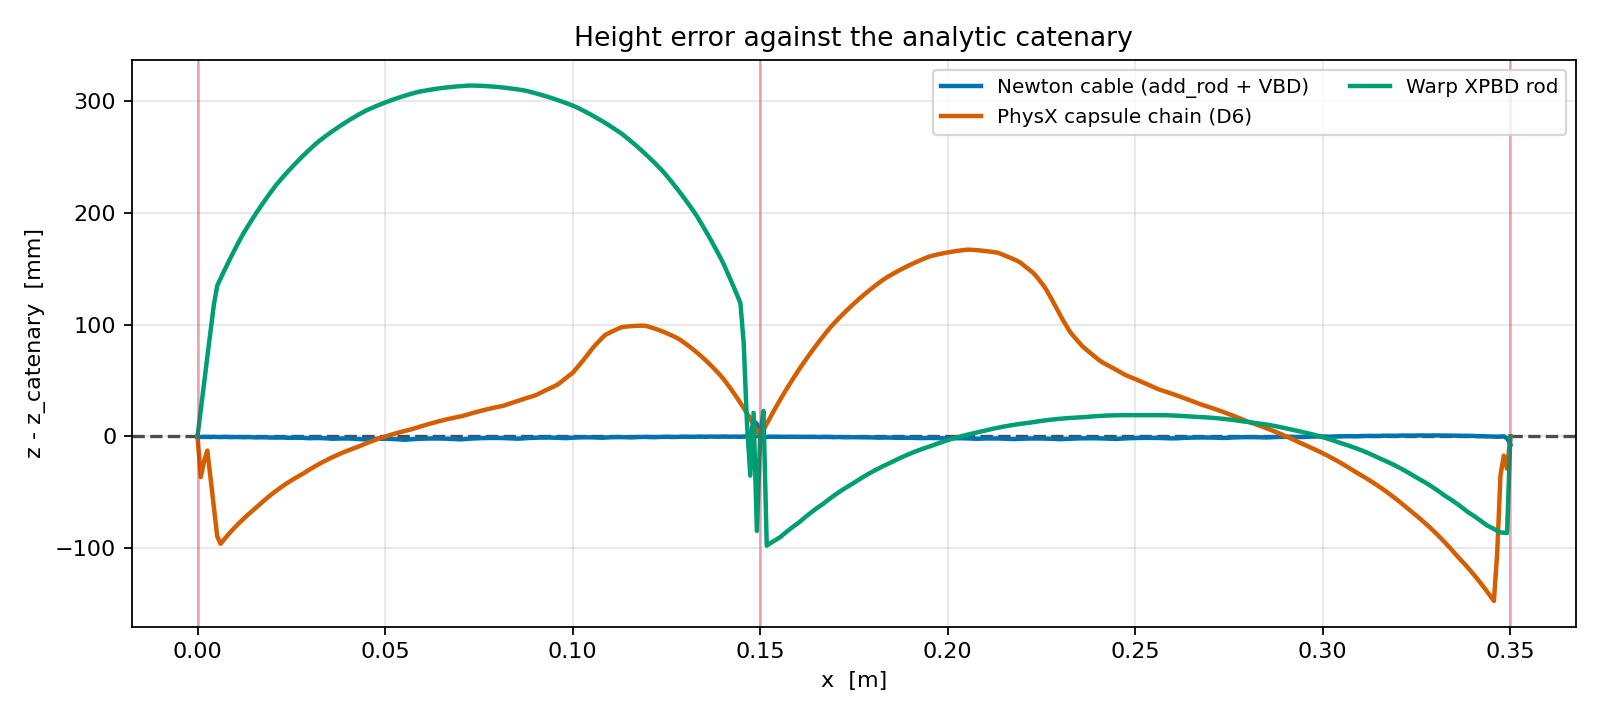
\includegraphics[width=\linewidth]{errors.png}
  \caption{Deviation from the analytic catenary along the cable.}
  \label{fig:errors}
\end{figure}


\begin{table}[htbp]
\centering\small
\begin{tabular}{lrr}
\toprule
method & RMSE vs photo [mm] & max [mm] \\
\midrule
    Newton cable (add\_rod + VBD) & 75.04 & 157.96 \\
    PhysX capsule chain (D6) & 34.34 & 138.38 \\
    Warp XPBD rod & 195.53 & 331.51 \\
\bottomrule
\end{tabular}
\caption{Simulation against the photographed cable. The extraction's frame is calibrated on the two outer clamps, which are level in the apparatus; the middle clamp is recovered to within 14~mm as an independent check (Section~\ref{sec:validity}), which bounds the accuracy of these figures.}
\end{table}

\section{Solver hyperparameters}

Every cable example shipped with Newton uses $10$ substeps and $5$ iterations.
Applied to this problem that is far too coarse; but the repository's previous
default of $8 \times 200$ was tuned by varying iterations alone, leaving the
substep axis untested. A sweep over both, scored against the analytic curve,
shows accuracy to be essentially a function of the \emph{product} --- while
cost is not, because each substep carries fixed overhead that an iteration does
not. Fewer substeps with more iterations is therefore strictly cheaper at equal
accuracy.

Separately, damping the stretch constraint proved actively harmful: it opposes
the solver's own length correction, and raising it to $10^{-2}$ cost roughly a
factor of six in accuracy for no benefit. Damping the \emph{bending}
constraint, by contrast, changed nothing measurable over a $600\times$ range,
because this cable's $EI$ is small enough that the bending mode carries almost
no energy.

\begin{table}[htbp]
\centering\small
\begin{tabular}{rrrrrr}
\toprule
substeps & iterations & budget & RMSE [mm] & arc drift [\%] & wall [s] \\
\midrule
    4 & 5 & 20 & 70.93 & 14.51 & 6.4 \\
    10 & 5 & 50 & 27.81 & 5.36 & 10.1 \\
    4 & 200 & 800 & 2.56 & 0.44 & 65.7 \\
    8 & 200 & 1600 & 1.53 & 0.22 & 190.1 \\
    10 & 200 & 2000 & 1.31 & 0.17 & 239.6 \\
    16 & 200 & 3200 & 2.09 & 0.12 & 379.7 \\
\bottomrule
\end{tabular}
\caption{Selected configurations from the sweep.}
\end{table}


\begin{figure}[htbp]
  \centering
  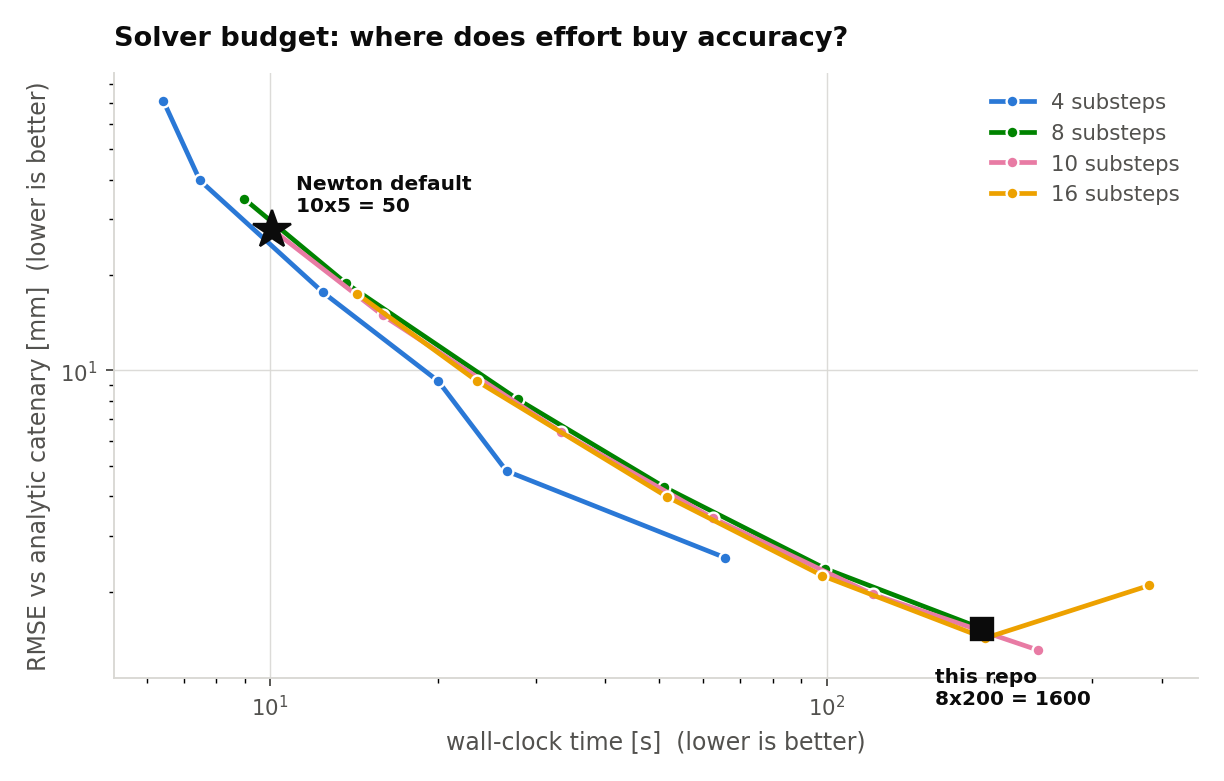
\includegraphics[width=\linewidth]{budget.png}
  \caption{Accuracy against wall-clock cost. Both axes logarithmic; the knee is where further cost stops buying accuracy.}
  \label{fig:budget}
\end{figure}



\begin{figure}[htbp]
  \centering
  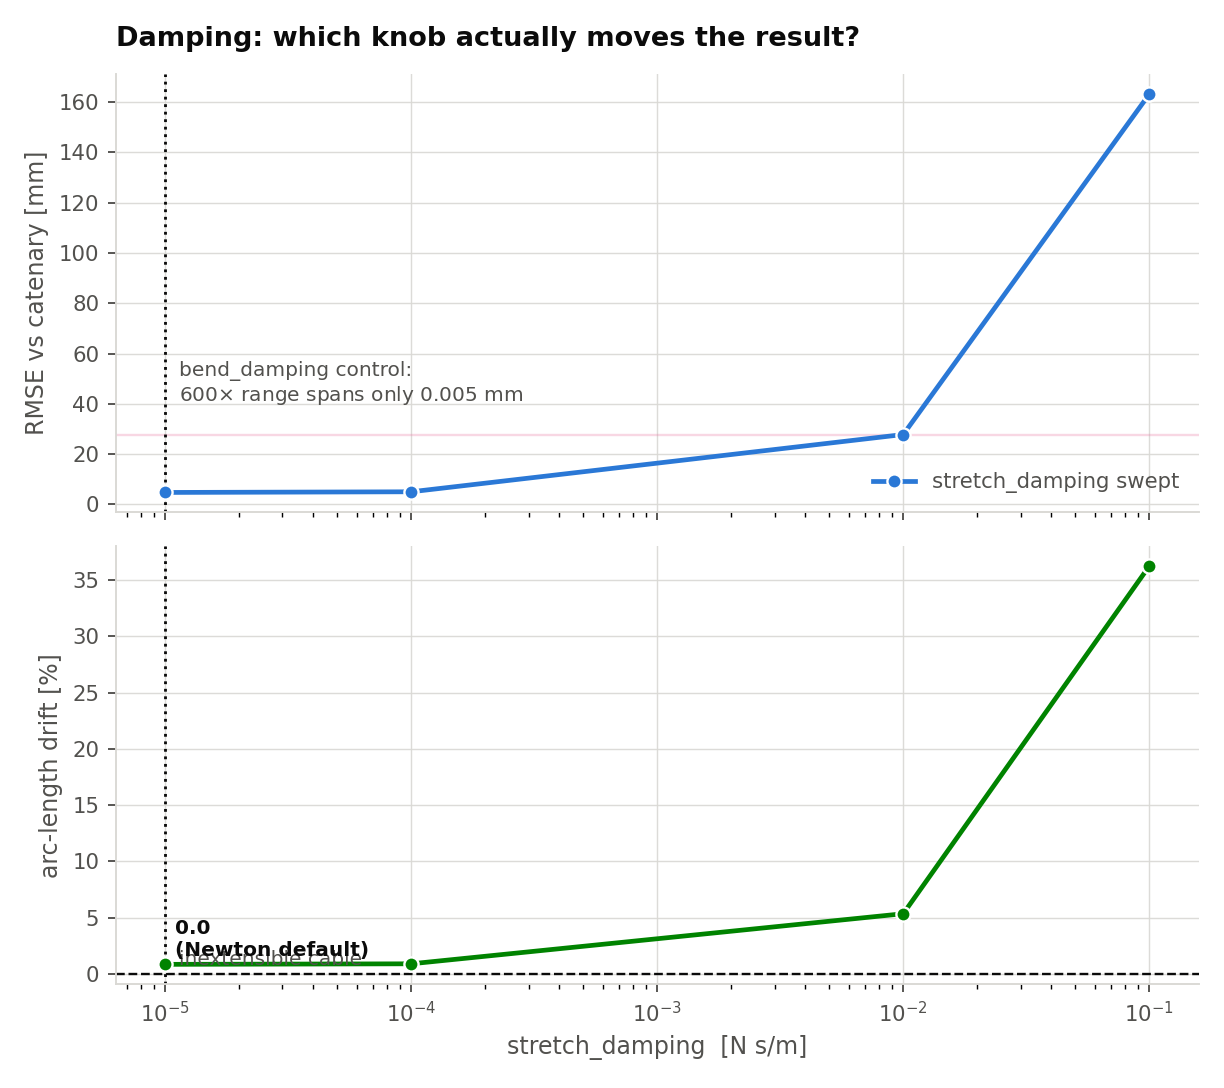
\includegraphics[width=\linewidth]{damping.png}
  \caption{Damping. Stretch damping dominates; the bend-damping control spans a 600x range and does nothing.}
  \label{fig:damping}
\end{figure}


\section{Provenance of the inputs}

\begin{table}[htbp]
\centering\small
\begin{tabular}{lll}
\toprule
field & source & value \\
\midrule
    \texttt{cable.length\_m} & measured & 0.8932 \\
    \texttt{supports.mid\_fraction} & measured & 0.4688 \\
\bottomrule
\end{tabular}
\caption{Which inputs were measured from the photograph and which were
assumed. Recorded automatically for every run.}
\end{table}

\section{Validity}
\label{sec:validity}

\paragraph{Frame calibration.} The cable's two ends are located
geodesically --- breadth-first search across the mask itself, twice --- rather
than as its leftmost and rightmost pixels. The distinction matters here: the
tape clamps the cable's \emph{angle} as well as its position, so a slack
cable leaves the clamp along the tape's direction and bends back, carrying it
horizontally \emph{past} its own anchor (86\,px in this photograph). Taking
the horizontal extreme therefore picks a point on the descending cable rather
than the clamp.

An earlier version did exactly that at one end while the other came from where
tracing halted --- two ends defined by two different rules --- and the
resulting frame was tilted enough to place two physically level clamps 81\,mm
apart in height. With both ends found by one rule, and the clamp-to-clamp line
adopted as the horizontal (the clamps are level in the apparatus, so this also
removes camera roll, here $-0.40^\circ$), that difference is now $0.0$\,mm by
construction.

\paragraph{Independent check.} The frame is fixed by the two OUTER clamps
alone, so the middle clamp is free to disagree, and is therefore a genuine
test. It is recovered at $x = 0.164$\,m against $0.150$\,m measured by tape ---
$14$\,mm, or 4\% of the span --- and $3.9$\,mm above the outer clamps against
$0$ expected. Neither is forced by the calibration. The residual is consistent
with hand-measuring the clamp positions and with lens distortion toward the
frame edges, and it bounds the accuracy of any
simulation-versus-photograph comparison below.

\paragraph{What the model-free check says.} The traced arc length exceeds the
length implied by fitting catenaries to the measured sags by roughly 58\,mm.
This is not numerical: it is the clamped end again. A catenary meets its
support at whatever angle the length demands, while the tape forces a
different angle and the cable bends to accommodate it, and that bend costs arc
length the catenary does not spend. It is the largest single modelling
discrepancy in this study and is a property of the apparatus, not of any
solver.

\noindent Independent of the photograph entirely:
\begin{itemize}
  \item the verification of~\eqref{eq:catenary} against its closed form;
  \item every solver's error against the analytic catenary;
  \item the hyperparameter sweep and its conclusions;
  \item the observation that the Warp rod diverges at this slackness, rising
        above the clamps rather than hanging between them.
\end{itemize}

\paragraph{Modelling limits.} The catenary is the $EI \to 0$ limit. The real
cable is a charger cable with a permanent set, so its rest shape is not
straight and some deviation from any ideal curve is physical rather than
numerical. The tape also clamps the cable's angle, which the classical
catenary does not model. Both effects are concentrated near the clamps, and
both are measurable once the frame is corrected --- which makes them results to
quantify rather than caveats to apologise for.

\end{document}
